\documentclass[a4paper]{article}
\usepackage{graphicx}
\usepackage{amsmath,amssymb,amstext}


\begin{document}

\subsubsection{CompareChildrenSimilar}

  \begin{description}
  
  \item[testcase\_01:] 2 Gleiche Modelle.Alle Kinder gematched
    
   \begin{equation*}
   Similarity = \frac{1+1+1}{3}=1
   \end{equation*}

  
    
	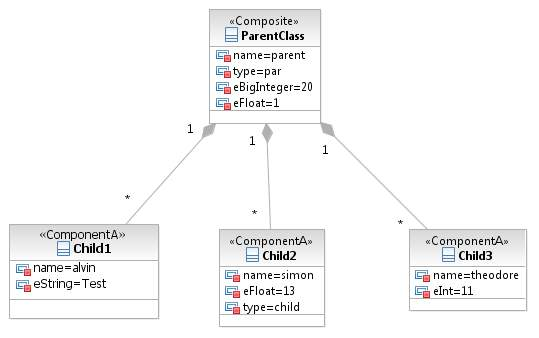
\includegraphics[scale=0.5]{CompareChildrenMatchedOrSimilarTestScreens/Testcase01model1.jpeg}
	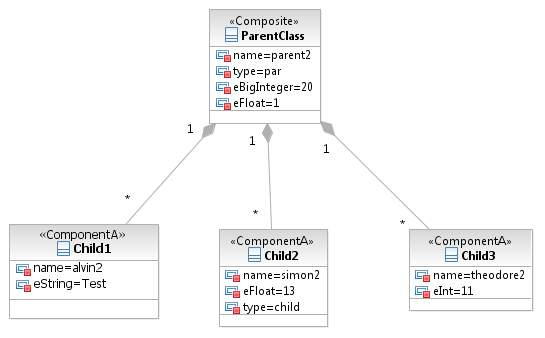
\includegraphics[scale=0.5]{CompareChildrenMatchedOrSimilarTestScreens/Testcase01model2.jpeg}

  \item[testcase\_02:]  Kein Matching bei den Kindern.
    
   \begin{equation*}
   Similarity = \frac{0+0+0}{3}=0
   \end{equation*}
    
	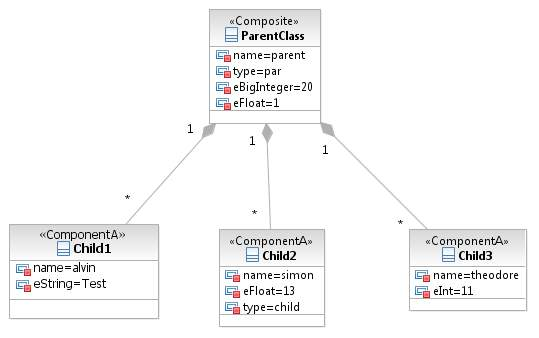
\includegraphics[scale=0.5]{CompareChildrenMatchedOrSimilarTestScreens/Testcase01model1.jpeg}
	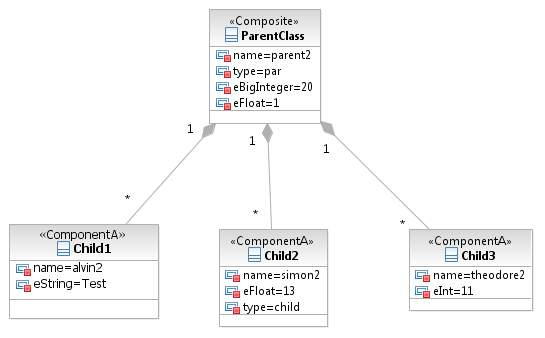
\includegraphics[scale=0.5]{CompareChildrenMatchedOrSimilarTestScreens/Testcase01model2.jpeg}

  \item[testcase\_03:] 2 von 3 Kindern sind gematched.
    
   \begin{equation*}
   Similarity = \frac{1+1+0}{3}=\frac{2}{3}
   \end{equation*}
    
	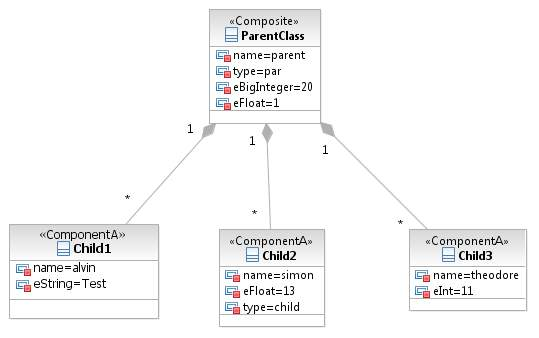
\includegraphics[scale=0.5]{CompareChildrenMatchedOrSimilarTestScreens/Testcase03model1.jpeg}
	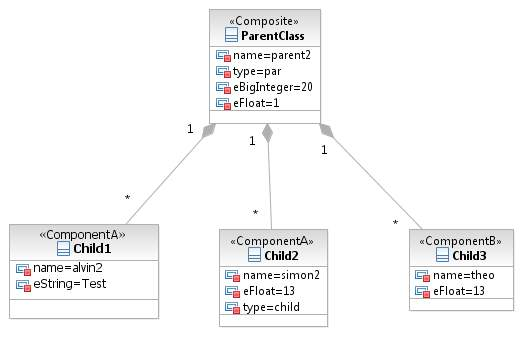
\includegraphics[scale=0.5]{CompareChildrenMatchedOrSimilarTestScreens/Testcase03model2.jpeg}

  \item[testcase\_04:]  2 von 3 Kindern sind gematched.
    
   \begin{equation*}
   Similarity = \frac{1+1+0}{3}=\frac{2}{3}
   \end{equation*}
    
	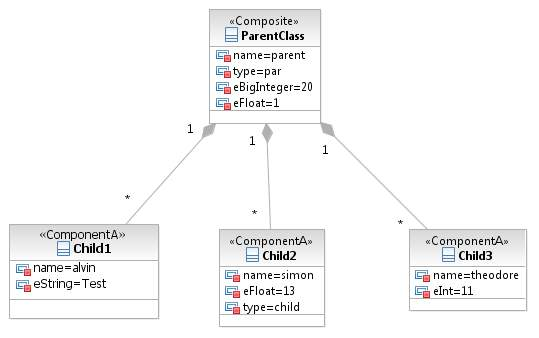
\includegraphics[scale=0.5]{CompareChildrenMatchedOrSimilarTestScreens/Testcase03model1.jpeg}
	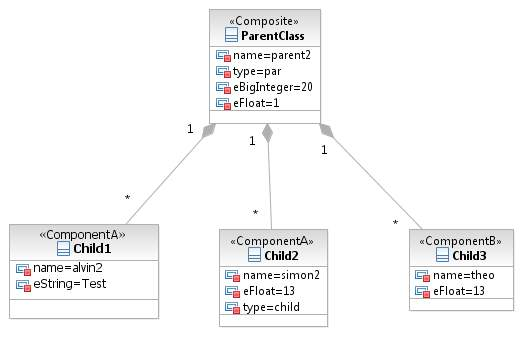
\includegraphics[scale=0.5]{CompareChildrenMatchedOrSimilarTestScreens/Testcase03model2.jpeg}

  \item[testcase\_05:]  2 Kinder sind gematched. 1 Kind fehlt (vergleich NULL).
    
   \begin{equation*}
   Similarity = \frac{1+1+0}{3}=\frac{2}{3}
   \end{equation*}
    
	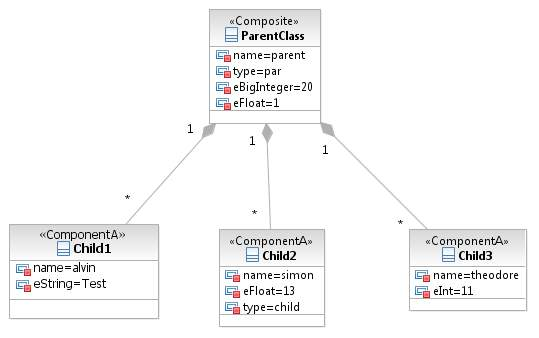
\includegraphics[scale=0.5]{CompareChildrenMatchedOrSimilarTestScreens/Testcase05model1.jpeg}
	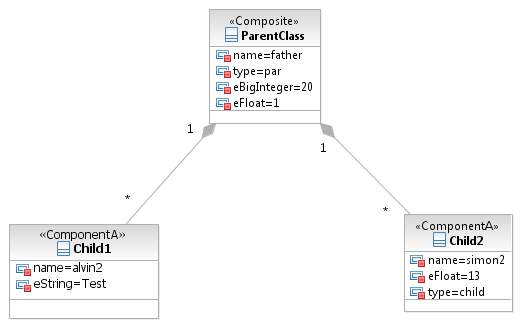
\includegraphics[scale=0.5]{CompareChildrenMatchedOrSimilarTestScreens/Testcase05model2.jpeg}

  \item[testcase\_06:]  2 Kinder sind gematched. 1 Kind fehlt (vergleich NULL).
    
   \begin{equation*}
   Similarity = \frac{1+1+0}{3}=\frac{2}{3}
   \end{equation*}
    
	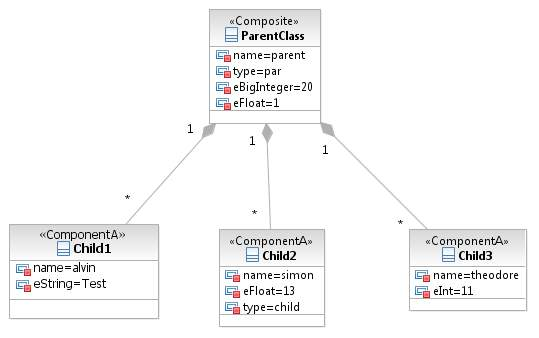
\includegraphics[scale=0.5]{CompareChildrenMatchedOrSimilarTestScreens/Testcase05model1.jpeg}
	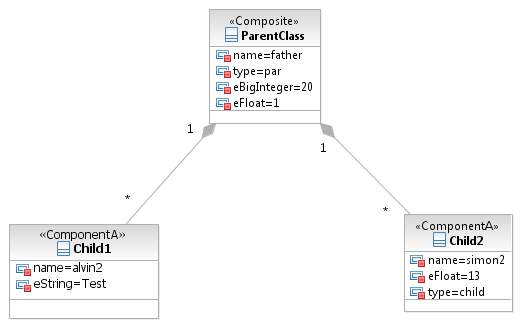
\includegraphics[scale=0.5]{CompareChildrenMatchedOrSimilarTestScreens/Testcase05model2.jpeg}

  \item[testcase\_07:]  2 von 3 Kindern sind gematched.
    
   \begin{equation*}
   Similarity = \frac{1+1+0}{3}=\frac{2}{3}
   \end{equation*}
    
	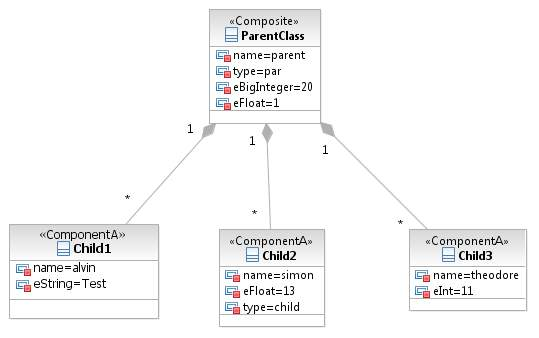
\includegraphics[scale=0.5]{CompareChildrenMatchedOrSimilarTestScreens/Testcase07model1.jpeg}
	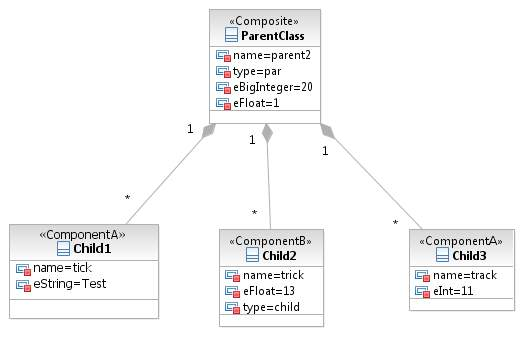
\includegraphics[scale=0.5]{CompareChildrenMatchedOrSimilarTestScreens/Testcase07model2.jpeg}

  \item[testcase\_08:]  2 von 3 Kindern sind gematched.
    
   \begin{equation*}
   Similarity = \frac{1+1+0}{3}=\frac{2}{3}
   \end{equation*}
       
	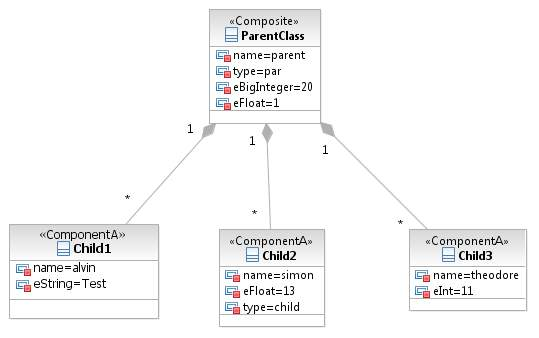
\includegraphics[scale=0.5]{CompareChildrenMatchedOrSimilarTestScreens/Testcase07model1.jpeg}
	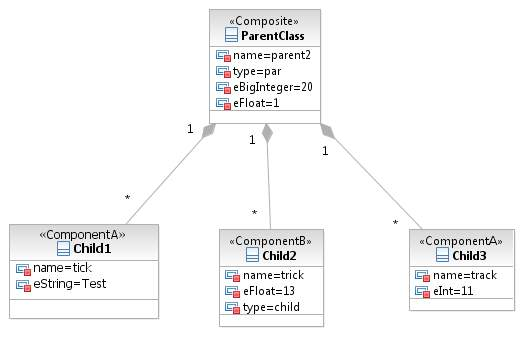
\includegraphics[scale=0.5]{CompareChildrenMatchedOrSimilarTestScreens/Testcase07model2.jpeg}

  \item[testcase\_09:]  Kein Matching bei den Kindern.
    
   \begin{equation*}
   Similarity = \frac{0+0+0}{3}=0
   \end{equation*}
    
	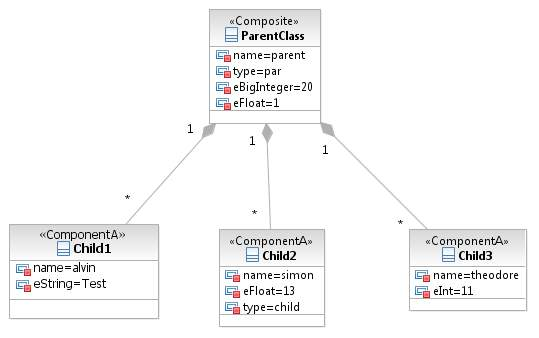
\includegraphics[scale=0.5]{CompareChildrenMatchedOrSimilarTestScreens/Testcase09model1.jpeg}
	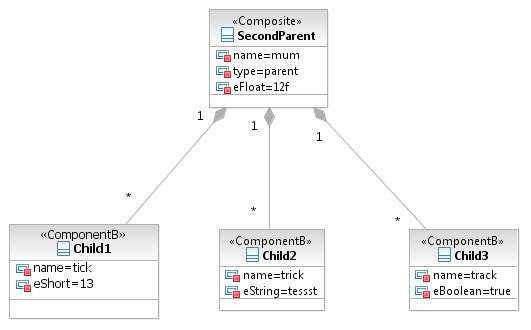
\includegraphics[scale=0.5]{CompareChildrenMatchedOrSimilarTestScreens/Testcase09model2.jpeg}

  \item[testcase\_10:]  Kein Matching bei den Kindern.
    
   \begin{equation*}
   Similarity = \frac{0+0+0}{3}=0
   \end{equation*}
    
	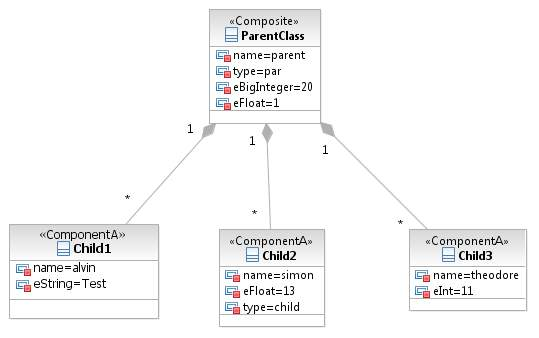
\includegraphics[scale=0.5]{CompareChildrenMatchedOrSimilarTestScreens/Testcase09model1.jpeg}
	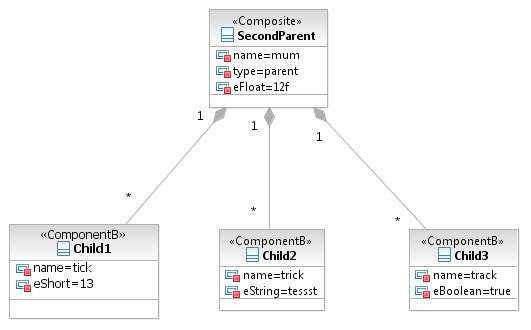
\includegraphics[scale=0.5]{CompareChildrenMatchedOrSimilarTestScreens/Testcase09model2.jpeg}
	\end{description}
	
	



\end{document}